\section{Definisi \textit{Micro Frameworki}}

\textit{Microframework} adalah istilah yang digunakan untuk merujuk pada kerangka kerja web minimalis. Kerangka ini sangat berbeda dengan kerangka kerja tumpukan penuh. Juga tidak memiliki sebagaian besar fungsionalitas yang umum yang ada dalam kerangka kerja aplikasi web lengkap, seperti:
\begin{enumerate}
\item Akun, otentikasi, otorisasi, peran, dll.
\item Abtraksi basis data melalui pemetaan objek-relasional.
\item Validai  \textit{input} dan sanitasi \textit{input}.
\item Mesin \textit{template web}.
\end{enumerate}

Biasanya, sebuah \textit{microframework} memfasilitasi menerima permintaan HTTP, merutekan permintaan HTTP ke \textit{controller} yang sesuai, mengirim \textit{controller}, dan mengembalikan respons HTTP. \textit{Microframeworks} seringkali dirancang khusus untuk membangun API untuk layanan atau aplikasi lain. Misalnya, Lumen \textit{microframework} dirancang untuk pengembangan \textit{Microservices} dan pengembangan API. \textit{Microframework}, sebuah \textit{tool} yang digunakan untuk \textit{project} yang lebih kecil dan penggunaan untuk kasus yang spesifik. Ini sama saja dengan menyederhanakan \textit{framework} agar lebih mudah dalam implementasi dan menyediakan \textit{testing} dan \textit{deployment} yang lebih cepat. \textit{Microframework} mengeluarkan banyak sekali komponen yang ada pada pengaturanan \textit{full-stack}, termasuk:
\begin{enumerate}
\item \textit{Web template engine}
\item \textit{Input validation}
\item \textit{Database abstraction}
\item \textit{Roles, accounts, and authentication}
\end{enumerate}

Kerugian menggunakan  \textit{microframework} adalah saat  \textit{project} mulai tumbuh besar dengan cepat. Dimana  \textit{microframework} tidak memiliki fitur yang dibutuhkan untuk mengakomodasi pertumbuhan  \textit{website}. Dengan kata lain kamu kehilangan fleksibelitas.  \textit{Micro-framework} lebih baik saat digunakan untuk  \textit{project} kecil yang membutuhkan kesederhanaan,  \textit{overhead} yang rendah dan  \textit{deployment} yang cepat.  \textit{Developer} yang sudah berpengalaman bisa saja menggunakan  \textit{microframework} pada awal  \textit{project} dan menambahkan tambahan  \textit{microframework} jika diperlukan. Hal ini merupakan pilihan yang menarik, tetapi untuk pemula dan  \textit{developer} menengah harus menghindari ini \cite{fadhilnet}.

\section{Jenis-Jenis \textit{Framework} Python serta Kelebihan dan Kekurangan}

\subsection{Django}

Django adalah kerangka kerja web Python yang memungkinkan individu dalam pengembangan yang bersih dan cepat. Kerangka kerja web secara umum dikatakan sebagai campuran komponen yang membantu pengembang mengembangkan situs web lebih cepat dan mudah. Karena itu, ini adalah kerangka kerja sumber bebas dan terbuka. Ini dapat disebut sebagai kerangka kerja yang memungkinkan pengembang untuk mengambil konsep penyelesaian secepat mungkin. Django sebagai kerangka kerja membantu mengurangi beberapa kesalahan keamanan umum yang dapat diawasi dengan mudah saat mengembangkan aplikasi. Skalabilitas adalah fitur lain yang disediakan oleh kerangka ini.

Django memiliki \textit{tagline "The web framework for perfectionists with deadlines"}, bagaimana tidak, karena secara \textit{default} Django sudah memiliki berbagai modul umum yang biasa digunakan ketika mengembangkan aplikasi web.

Kelebihan:
\begin{enumerate}
\item Cepat.

Ini telah dirancang sedemikian rupa untuk membantu pengembang membuat aplikasi secepat mungkin. Dari ide, produksi hingga rilis, Django membantu menjadikannya efektif dan efisien. Dengan demikian itu menjadi solusi ideal bagi pengembang yang memiliki fokus utama pada tenggat waktu.

\item Penuh dimuat.

Ini bekerja dengan cara yang mencakup puluhan tambahan untuk membantu dengan otentikasi pengguna, peta situs, administrasi konten, umpan RSS, dan banyak lagi hal-hal seperti itu. Aspek-aspek ini membantu dalam melaksanakan proses pengembangan web sepenuhnya.

\item Aman.

Ketika melakukannya di Django, dipastikan bahwa pengembang tidak melakukan kesalahan yang terkait dengan keamanan. Beberapa kesalahan umum termasuk injeksi SQL, pemalsuan permintaan lintas situs, clickjacking dan skrip lintas situs. Untuk mengelola nama pengguna dan kata sandi secara efektif, sistem otentikasi pengguna adalah kuncinya.

\item Dapat diukur.

Untuk memenuhi permintaan lalu lintas terberat, manfaat kerangka Django dapat dilihat. Oleh karena itu, situs tersibuk menggunakan media ini untuk dengan cepat memenuhi permintaan lalu lintas.

\item Serbaguna.

Manajemen konten,\textit{ platform} komputasi ilmiah, dan bahkan organisasi besar, semua aspek ini dikelola secara efisien dengan penggunaan Django.

\item Dokumentasi yang sangat lengkap dan kamu tidak perlu banyak - banyak \textit{googling} karena sudah disediakan contoh.
\item Modul administrasi yang \textit{auto generate} sesuai dengan model yang didefinisikan di dalam aplikasi. Lebih dari sekedar \textit{CRUD generator}.
\item Sistem migrasi \textit{database} otomatis yang tidak perlu kamu tulis \textit{script}-nya. Cukup mengubah class dan struktur \textit{database} pun berubah sesuai perubahan terakhir.
\item Memiliki sistem form yang kokoh.
\item Sudah \textit{built-in} untuk sistem autentikasi dan roles bila Anda menggunakan \textit{relational database} yang didukung Django seperti MySQL dan PostgreSQL.
\item Memiliki ekstensi - ekstensi yang bisa membuat kamu lebih produktif seperti \textit{Django Rest Framework, Django Rest Auth, Django Celery, Django Mongoengine, GeoDjango,} dan lainnya.
\item Memiliki \textit{template engine} sendiri yang lebih \textit{powerful}.
\item Kompatibilitas dengan berbagai modul dan \textit{library} lain.
\end{enumerate}

Kekurangan:
\begin{enumerate}
\item Menggunakan pola perutean, tentukan URL-nya
\item Django terlalu monolitik
\item Semuanya didasarkan pada Django ORM
\item Komponen dikerahkan bersama
\item Pengetahuan tentang sistem lengkap diperlukan untuk bekerja.
\end{enumerate}

\section{Instalasi dan Hello World di Flask}

\subsection{Instalasi Python 2.7.}

Mulai dengan tutorial dalam menginstall Python 2.7. Python ini digunakan untuk \textit{code} pembaca data dari sinyal gelombang otak yang telah dihasilkan oleh alat EEG yaitu NeuroSky Mindwave. Baiklah langsung kita mulai saja:
\begin{enumerate}
\item Pertama-tama silahkan download software dari python versi 2 di laptop anda. Download python versi 2.7.15 dari situs web resminya yaitu https://www.python.org/. Silahkan sesuaikan dengan kapasitas laptop anda, bisa yang win 32 atau yang win 64 (32 bit / 64 bit). Contoh downloadnya seperti pada gambar \ref{fig:python}.
\begin{figure}[!htbp]
	\centerline{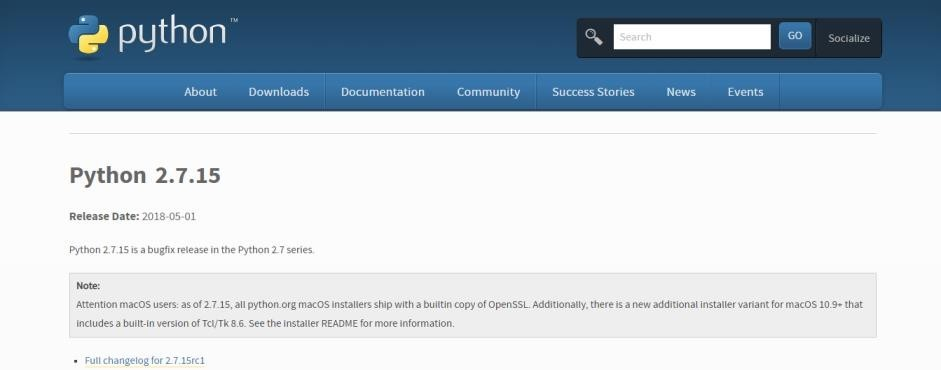
\includegraphics[width=1\textwidth]{figures/8/python.jpg}}
	\caption{Download Softfile Python 2.7.}
	\label{fig:python}
\end{figure}

\item Setelah di \textit{download}  silahkan  buka  Command  Prompt  di komputer/PC anda.
\item Kemudian silahkan ketikkan perintah \verb|pip install flask|.
\item Setelah mengetikkan perintah tersebut, silahkan tekan \textit{enter} maka prosesnya akan berjalan. Silahkan tunggu hasilnya. Hasilnya akan nampak seperti gambar \ref{fig:cek_python}.
\begin{figure}[!htbp]
	\centerline{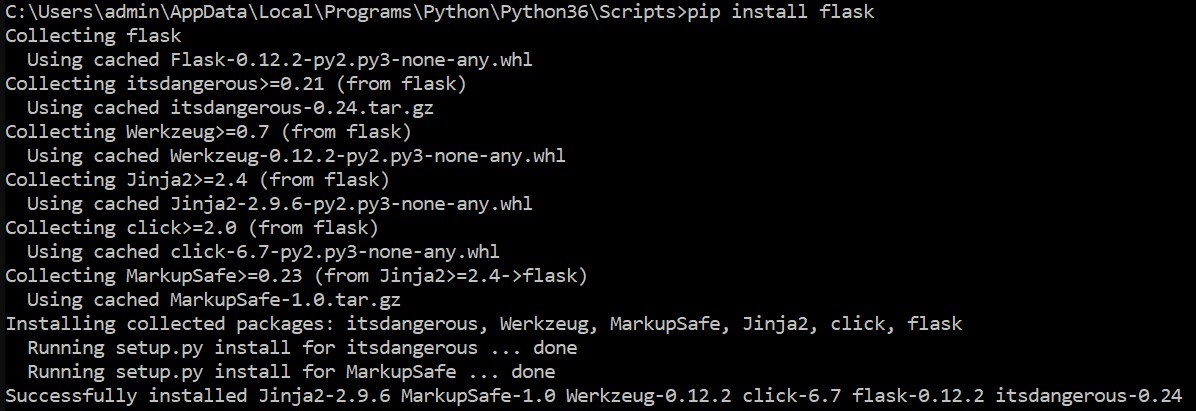
\includegraphics[width=1\textwidth]{figures/8/cek_python.jpg}}
	\caption{Froses Instalasi Flask}
	\label{fig:cek_python}
\end{figure}

\end{enumerate}

Perintah python flask. Contoh \textit{source code} seperti pada listing \ref{lst:hello}.
\lstinputlisting[caption=Contoh kode program hello.py, label={lst:hello}]{src/8/hello.py}
 Contoh \textit{source code} main.py seperti pada listing \ref{lst:main}.
\lstinputlisting[caption=Contoh kode program main.py, label={lst:main}]{src/8/main.py}
